%tex root = thesis.tex

\chapter{Praktische Aspeckte}
\label{chapter-aspeckte}
Asymmetrische Kryptosysteme haben den Vorteil, dass sie das Geheimnis möglichst klein halten, da jeder Benutzer nur seinen eigenen privaten Schlüssel geheim halten muss. Im Gegensatz dazu muss bei einem symmetrischen Kryptosystem jeder Benutzer alle Schlüssel geheim halten, was einen mit zunehmender Benutzerzahl steigenden Aufwand bedeutet.\ref{abc}
Im Vergleich zu symmetrischen Algorithmen arbeiten die asymmetrischen Algorithmen sehr langsam. In der Praxis wird dieses Problem auf unterschiedliche Weise umgangen. Zur Verschlüsselung werden hybride Verfahren eingesetzt, bei denen lediglich ein symmetrischer Schlüssel mit dem asymmetrischen Verfahren verschlüsselt wird und die eigentliche Nachricht mit diesem symmetrischen Schlüssel. Bei digitalen Signaturen wird in der Regel statt einer Nachricht nur deren Hashwert signiert.\ref{abcd}
\begin{figure*}
	\label{abc}
	\begin{center}
		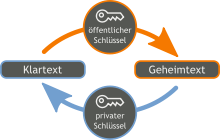
\includegraphics[width=5cm]{abcde.png}	
	\end{center}
	\caption{Verschlüsselung mit öffentlichem Schlüssel und Entschlüsselung mit privatem Schlüssel}
	
\end{figure*}
\begin{figure*}
	\label{abcd}
	\begin{center}
		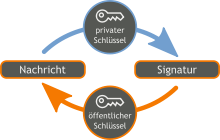
\includegraphics[width=5cm]{ab.png}	
	\end{center}
	\caption{Signieren mit privatem Schlüssel und Verifikation mit öffentlichem Schlüssel}
	
\end{figure*}


\section{Hybride Verschlüsselung}
Unter Hybrider Verschlüsselung versteht man eine Kombination aus asymmetrischer Verschlüsselung und symmetrischer Verschlüsselung. Dabei wählt der Sender einen zufälligen symmetrischen Schlüssel, der Session-Key genannt wird. Mit diesem Session-Key werden die zu schützenden Daten symmetrisch verschlüsselt. Anschließend wird der Session-Key asymmetrisch mit dem öffentlichen Schlüssel des Empfängers verschlüsselt. Dieses Vorgehen löst das Schlüsselverteilungsproblem und erhält dabei den Geschwindigkeitsvorteil der symmetrischen Verschlüsselung.

\section{Hashwert}
Eine kryptologische Hashfunktion oder kryptographische Hashfunktion ist eine spezielle Form der Hashfunktion, welche kollisionsresistent sein sollte und nach Definition immer eine Einwegfunktion ist.
Eine Hashfunktion ist eine Funktion, die eine Zeichenfolge beliebiger Länge auf eine Zeichenfolge mit fester Länge abbildet. Mathematisch ist diese Funktion nicht injektiv (linkseindeutig) und nicht notwendigerweise surjektiv (rechtstotal).
Anwendungen von kryptologischen Hashfunktionen sind vor allem die Datenverarbeitung, zur Integritätsprüfung von Dateien oder Nachrichten. Darüber hinaus werden sie eingesetzt zur Verschleierung von Passwortdateien, als Datenbasis digitaler Signaturen, als Pseudo-Zufallszahlengeneratoren oder zur Konstruktion von Blockchiffren.
Inhaltsverzeichnis.


